\section{Exercises}

\begin{frame}[allowframebreaks]
    \frametitle{Outline}
    \tableofcontents[currentsection, currentsubsection]
\end{frame}

\begin{frame}
    \frametitle{WMA Problem 2.5a \& 2.6a}
        \begin{verse}
            The Williams family's income of \$25,000 falls below 185\% of the 
            \href{http://aspe.hhs.gov/poverty/12poverty.shtml}{Federal Poverty
            Threshold} for a family of four, qualifying them
            for food stamps. 
        \end{verse}
        \vskip0.3in
\begin{description}
    \item[Problem 2.5a] {Identify terms that need to be defined or restated
        for a nontechnical audience}
    \item[Problem 2.6a] Rewrite the sentences in the previous questions for an
        audience with a fifth-grade education.  Convey the main point,
        not the calculation or the jargon. 
    \item[FYI] \href{http://www.bloomberg.com/video/how-the-rich-get-richer-and-the-poor-poorer-kfuILNN9SoaQXLd5cVBwPQ.html}{Off-the-chart}
\end{description}
\end{frame}

\begin{frame}
    \frametitle{WMA Problem 2.8a}
    Rewrite each of these sentences to specify the direction and magnitude of
    the association:
    \vskip0.1in
    \begin{center}
    \begin{verse}
        In the United States, race is correlated with income. 
    \end{verse}
    \end{center}
    \begin{table}
        \centering
        \caption{\textbf{Median income by race and Hispanic origin, United States, 1999}}
        \label{tab:WMAex2x8}
        \begin{tabular}{lc}
        Race/Hispanic origin & Median Income \\
        \hline 
        White   & \$42,504 \\
        Black   & \$27,910 \\ 
        Asian/Pacific Islander   & \$51,205 \\ 
        Hispanic (can be of any race) & \$30,735 \\
        \hline
        \end{tabular}
    \end{table}
\end{frame}

\begin{frame}
    \frametitle{WMA Problem 2.9}
    Use the GEE approach to describe the patterns in the figure below,
    including an introductory sentence about the purpose of the chart 
    before summarizing the patterns. 
    \begin{figure}
        \begin{center}
            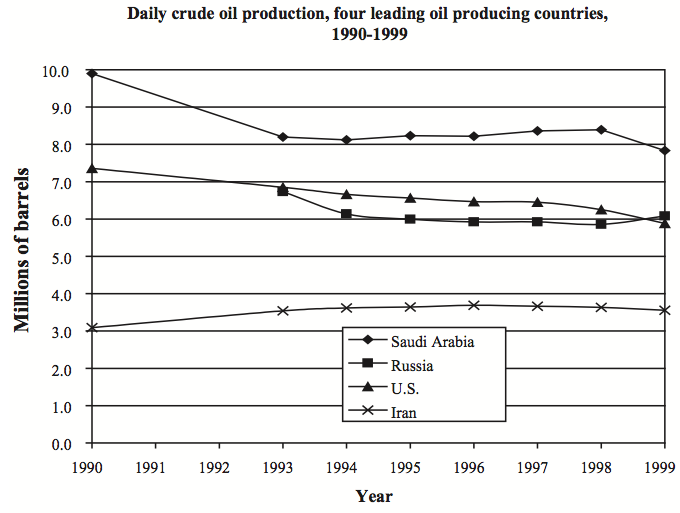
\includegraphics[width=0.6\textwidth]{images/WMAex2x9.png}
        \end{center}
    \end{figure}
\end{frame}

\begin{frame}
    \frametitle{IMM Problem 1.1}
    Suppose people enter the elevators in a skyscraper at random during the
    morning rush. The result will be several elevators stopping on each floor
    to discharge one or two passengers each. 
    \vskip0.1in
    \begin{itemize}
        \item Discuss schemes for improving the situation. 
        \item How could improvement be measured? 
        \item How could you model the situation to decide what scheme to adopt?
    \end{itemize}
\end{frame}

\begin{frame}
    \frametitle{IMM Problem 1.6}
    Unless you have been extremely lucky, you have had a large class in a
    poorly designed lecture hall. 
    
    \vskip0.25in
    \begin{description}
        \item[(a)] What are some criteria to be considered
    in designing a large lecture hall? 
    \end{description}
\end{frame}
    
\begin{frame}
    \frametitle{IMM Problem 1.6}
    Unless you have been extremely lucky, you have had a large class in a
    poorly designed lecture hall. 
    \vskip0.15in
    \begin{description}
        \item[(b)] One criterion is legibility of material written on the boards. 
        \begin{itemize}
            \item Construct a model of legibility as a function of 
                \begin{itemize}
                    \item  \emph{the distance} your seat is from the board 
                    \item \emph{the angle} at which you look at the board 
                \end{itemize}
            \item What will the curves of constant legibility look like on a
                floor plan?
            \item How can you test this prediction? Try it. 
            \item Does this suggest shaping the back of the hall differently
                than is usually done? How?
        \end{itemize}    
    \end{description}
    \vfill
\end{frame}
     
\begin{frame}
    \frametitle{IMM Problem 1.6}
    Unless you have been extremely lucky, you have had a large class in a
    poorly designed lecture hall. 
    
    \vskip0.25in
    \begin{description}
        \item[(c)] Can mathematical modeling help with any other criteria
    besides the one mentioned in (b)? Try to pick a criterion from among these
    possibilities and develop a model for it.
    \end{description}
\end{frame}



\newtheorem{POEMbender}{The Blind Men and the Elephant}
\begin{frame}[fragile]
    \frametitle{Collect All: \LaTeXs + Git}
    \begin{POEMbender}
        In-class Group Exercise (Scavenger hunt):
    \end{POEMbender}
        \begin{itemize}
            \item Start up a git folder,
            \item Create and edit the \texttt{.gitignore} file,
            \item Download the template for a beamer file,
            \item Look up the poem from the book,
            \item One slide per stanza,
            \item Use \texttt{verse} environment,
            \item Compile after each stanza,
            \item Commit after creating each stanza,
            \item Repeat until done.
        \end{itemize}
\end{frame}
